\chapter{Static Schedules}
\label{chap:Static}
This chapter largely follows the results of \citet{Pegden}. The aim is to derive a method for choosing an optimal static schedule. A static schedule is a sequence of $n$ customer arrival times $t_{1}, \ldots, t_{n}$ chosen at the start of service and fixed for the duration of service. 

For simplicity, these results assume the customer service times are independent and identically distributed (iid) exponential random variables with mean $\mu$. There is a single server. All customers are punctual and arrive at their scheduled arrival time.

\section{Objective Function}
The optimal schedule minimises the expected cost, which is a linear combination of the expected total customers' waiting time and the expected server availability time.

Denote the expected waiting time of customer $i$ as $w_{i}$. The expected total customers' waiting time is the sum of the individual customer's expected waiting times.
\begin{equation}
	\mathbb{E} \Big[\text{total customer's waiting time} \Big] = \sum_{i = 1}^{n} w_{i}
\end{equation}

Instead of solving for the customer arrival times, it is easier to solve for the arrival time of the first customer $t_{1}$ and the customer interarrival times $\mathbf{x}_{n} = (x_{1}, \ldots, x_{n - 1})$ where $x_{i} = t_{i + 1} - t_{i}$. The expected server availability time is the expected time from the start of service until the end of service. This time is the summation of the last customer's scheduled arrival time, the last customer's expected waiting time and the last customer's expected service time.
\begin{equation}
	\mathbb{E} \Big[\text{server availability time} \Big] = \left( t_{1} + \sum_{i = 1}^{n - 1} x_{i} \right) + w_{n} + \mu
\end{equation}

Denote $c_{W}$ and $c_{S}$ as the per unit time cost of the expected total customer's waiting time and the per unit time cost of the expected server availability time respectively. The objective function to be minimised is thus,
\begin{equation}
	\phi (t_{1}, \mathbf{x}_{n}) = c_{W} \sum_{i = 1}^{n} w_{i} + c_{S} \left[ t_{1} + \sum_{i = 1}^{n - 1} x_{i} + w_{n} + \mu \right]
\end{equation}

The first customer should obviously be scheduled for the start of service so $t_{1} = 0$. Moreover, can scale the objective function by dividing by $(c_{W} + c_{S})$ and defining $\gamma = \frac{c_{S}}{c_{W} + c_{S}}$.
\begin{equation}
	\phi (\mathbf{x}_{n}) \coloneqq (1 - \gamma) \sum_{i = 1}^{n} w_{i} + \gamma \left[ \sum_{i = 1}^{n - 1} x_{i} + w_{n} + \mu \right]
	\label{eqn:StaticObjective}
\end{equation}

The optimal static schedule is thus the interarrival times that minimise Equation~\ref{eqn:StaticObjective}

\section{Expected Waiting Time}
We want to express $w_{i}$ (i.e., the expected waiting time of customer $i$) as a function of the interarrival times $\mathbf{x}_{n}$. If there are $j$ customers in the system immediately prior to the arrival of customer $i$, then $w_{i} = j \mu$ by the memoryless property of the exponential distribution. The number of customers in the system refers to both customers being served and customers waiting for service.

Denote the number of customers in the system immediately prior to the arrival of customer $i$ by $N_{i}$. Thus, the expected waiting time of customer $i$ is given by
\begin{equation}
	w_{i} = \sum_{j = 0}^{i - 1} (j \mu) \mathbb{P} (N_{i} = j)
\end{equation}

It is more common in queuing theory to consider the queue length as a right-continuous process. This would involve considering the number of customers in the system on the arrival of the customer $i$. However, in this chapter, we choose to remain consistent with the notation of \citet{Pegden} and consider the system size as a left-continuous process.

\citet{Pegden} derive the following complicated recursive equation for calculating the probability of a given number of customers in the system.
\begin{equation}
	\mathbb{P} (N_{i} = j) = \begin{cases} 1 & \text{for $i = 1$, $j = 0$} \\
	\sum_{k = 1}^{i - 1} \mathbb{P} (N_{i - 1} = k - 1) \left[ 1 - \sum_{l = 0}^{k - 1} \frac{x_{i - 1}^{l}}{\mu^{l} l!} \mathrm{e}^{\frac{- x_{i - 1}}{\mu}}\right] & \text{for $i \geq 2$, $j = 0$} \\
	\sum_{k = 0}^{i - j - 1} \mathbb{P} (N_{i - 1} = j + k - 1) \left[ \frac{x_{i - 1}^{k}}{\mu^{k} k!} \mathrm{e}^{\frac{- x_{i - 1}}{\mu}} \right] & \text{for $i \geq 2$, $j \geq 1$} \end{cases}
	\label{eqn:StaticProbSystem}
\end{equation}

Pegden and Rosenshine's formulation can be solved more efficiently by identifying that $\{ N_{i} \}$ forms a discrete time Markov chain with nonstationary transition probabilities. \citet{Stein} show that the transition from $N_{i - 1}$ to $N_{i}$ is governed by the transition matrix
\begin{equation*}
	T (x_{i - 1}) = \kbordermatrix{
	& 0 & 1 & 2 & 3 & \ldots & n - 1 & n \\
	0 & r_{0} & a_{0} & 0 & 0 & \ldots & 0 & 0 \\
	1 & r_{1} & a_{1} & a_{0} & 0 & \ldots & 0 & 0 \\
	2 & r_{2} & a_{2} & a_{1} & a_{0} & \ldots & 0 & 0 \\
	\vdots & \vdots & \vdots & \vdots & \vdots & \ldots & \vdots & \vdots \\
	n - 1 & r_{n - 1} & a_{n - 1} & a_{n - 2} & a_{n - 3} & \ldots & a_{1} & a_{0} \\
	n & 0 & 0 & 0 & 0 & \ldots & 0 & 1
	}
\end{equation*}

where
\begin{align}
	\begin{split}
		a_{k} & = \frac{x_{i - 1}^{k}}{\mu^{k} k!} \mathrm{e}^{\frac{- x_{i - 1}}{\mu}} \\
		r_{k} & = 1 - \sum_{l = 0}^{k} a_{l}
	\end{split}
\end{align}

The last row of $T (x_{i - 1})$ is arbitrary as it is not possible to have $n$ customers in the system immediately before a customer's arrival.

Instead of Equation~\ref{eqn:StaticProbSystem}, for $i \geq 2$, the distribution of $N_{i}$ is more clearly expressed by
\begin{align}
	\begin{split}
		& \ \left( \begin{array}{ccc} \mathbb{P} (N_{i} = 0) & \ldots & \mathbb{P} (N_{i} = n) \end{array} \right) \\
		= & \ \left( \begin{array}{ccc} \mathbb{P} (N_{i - 1} = 0) & \ldots & \mathbb{P} (N_{i - 1} = n) \end{array} \right) T (x_{i - 1}) \\
		= & \ \left( \begin{array}{ccc} \mathbb{P} (N_{1} = 0) & \ldots & \mathbb{P} (N_{1} = n) \end{array} \right) T (x_{1}) T (x_{2}) \cdots T (x_{i - 1})
	\end{split}
\end{align}

The distribution of $N_{1}$ (i.e., the initial distribution) is given by
\begin{equation}
	\left( \begin{array}{ccc} \mathbb{P} (N_{1} = 0) & \ldots & \mathbb{P} (N_{1} = n) \end{array} \right) = \left( \begin{array}{cccc} 1 & 0 & \ldots & 0 \end{array} \right)
\end{equation}

Therefore, the expected waiting time of customer $i$ can be compactly expressed using the transition matrices as
\begin{equation}
	w_{i}
	= \left( \begin{array}{cccc} 1 & 0 & \ldots & 0 \end{array} \right)
	T (x_{1}) T (x_{2}) \cdots T (x_{i - 1})
	\left( \begin{array}{c} 0 \\ 1 \\ 2 \\ \vdots \\ n \end{array} \right)
	\label{eqn:StaticWaiting}
\end{equation}

\section{Example Models}
\subsection{Model for 2 Customers}
\label{sec:StaticTwoCust}
We consider the simplest case of this model where there are two customers to be scheduled (i.e., $n = 2$). As the first customer is scheduled to arrive at the start of service, the only unknown variable is the optimal interarrival time between the first and second customer (i.e., $x_{1}$).

By Equation~\ref{eqn:StaticWaiting}, the expected waiting times of the two customers are
\begin{equation}
	\begin{split}
		w_{1} & = 0 \\
		w_{2} & = \mu \mathrm{e}^{\frac{- x_{1}}{\mu}}
	\end{split}
\end{equation}

By Equation~\ref{eqn:StaticObjective}, the objective function to be minimised is given by
\begin{equation}
	\phi (x_{1}) = \mu \left[ \gamma + \exp \left( \frac{- x_{1}}{\mu} \right) \right] + \gamma x_{1}
\end{equation}

This objective function is convex as
\begin{equation}
	\forall x_{1} \ \ \phi'' (x_{1}) = \frac{1}{\mu} \exp \left( \frac{- x_{1}}{\mu} \right) > 0
\end{equation}

Due to the convexity of the objective function, the optimal policy that minmises $\phi (x_{1})$ can be found by solving:
\begin{equation}
	\phi' (x_{1}) = 0 \implies - \exp \left( \frac{- x_{1}}{\mu} \right) + \gamma = 0
\end{equation}

Therefore, the optimal policy is:
\begin{equation}
	x_{1}^{*} = \argmin_{x_{1} \geq 0} \phi (x_{1}) = - \mu \ln \gamma
\end{equation}

As the server availability cost increases relative to the customer waiting cost (i.e., $\gamma$ increases), the second customer is scheduled to arrive earlier (i.e., $x_{1}^{*}$ decreases).

Unfortunately, as \citet{Pegden} found, no general algebraic solution exists for more than two customers (i.e., $n \geq 3$). All other cases need to be solve numerically. Pegden and Rosenshine prove that the objective function $\phi (\mathbf{x}_{n})$ is convex for $n = 1, 2, 3, 4$. Moreover, they conjecture that it appears to be convex for general $n$, but are unable to prove it.

\subsection{Model for 15 Customers}
The more interesting cases concern scheduling a larger number of customers. We consider here the case of $n = 15$. Without loss of generality, can let $\mu = 1$. For $\mu \neq 1$, the solutions found are the optimal values of $\mu \mathbf{x}_{n} = (\mu x_{1}, \ldots, \mu x_{n - 1})$.

Minimising the objective function is a constrained optimization problem. A numeric solution to this problem can be found using the `L-BFGS-B' method of \newline $\texttt{scipy.optimize.minimize}$ in Python. The Broyden-Fletcher-Goldfarb-Shanno (BFGS) algorithm is an iterative method for solving an unconstrained optimization problem. The `L-BFGS-B' is an extension of the BFGS algorithm to handle simple bound constraints on the variables. For a more detailed explanation of the method, see \citet{Byrd}.

Figure~\ref{fig:Static_Time_Gamma} plots the optimal interarrival times $\mathbf{x}_{n}^{*} = (x_{1}^{*}, \ldots, x_{14}^{*})$ for scheduling $15$ customers with a mean service time $\mu = 1$ for various values of $\gamma$.
\begin{figure}[htb]
	\centering
	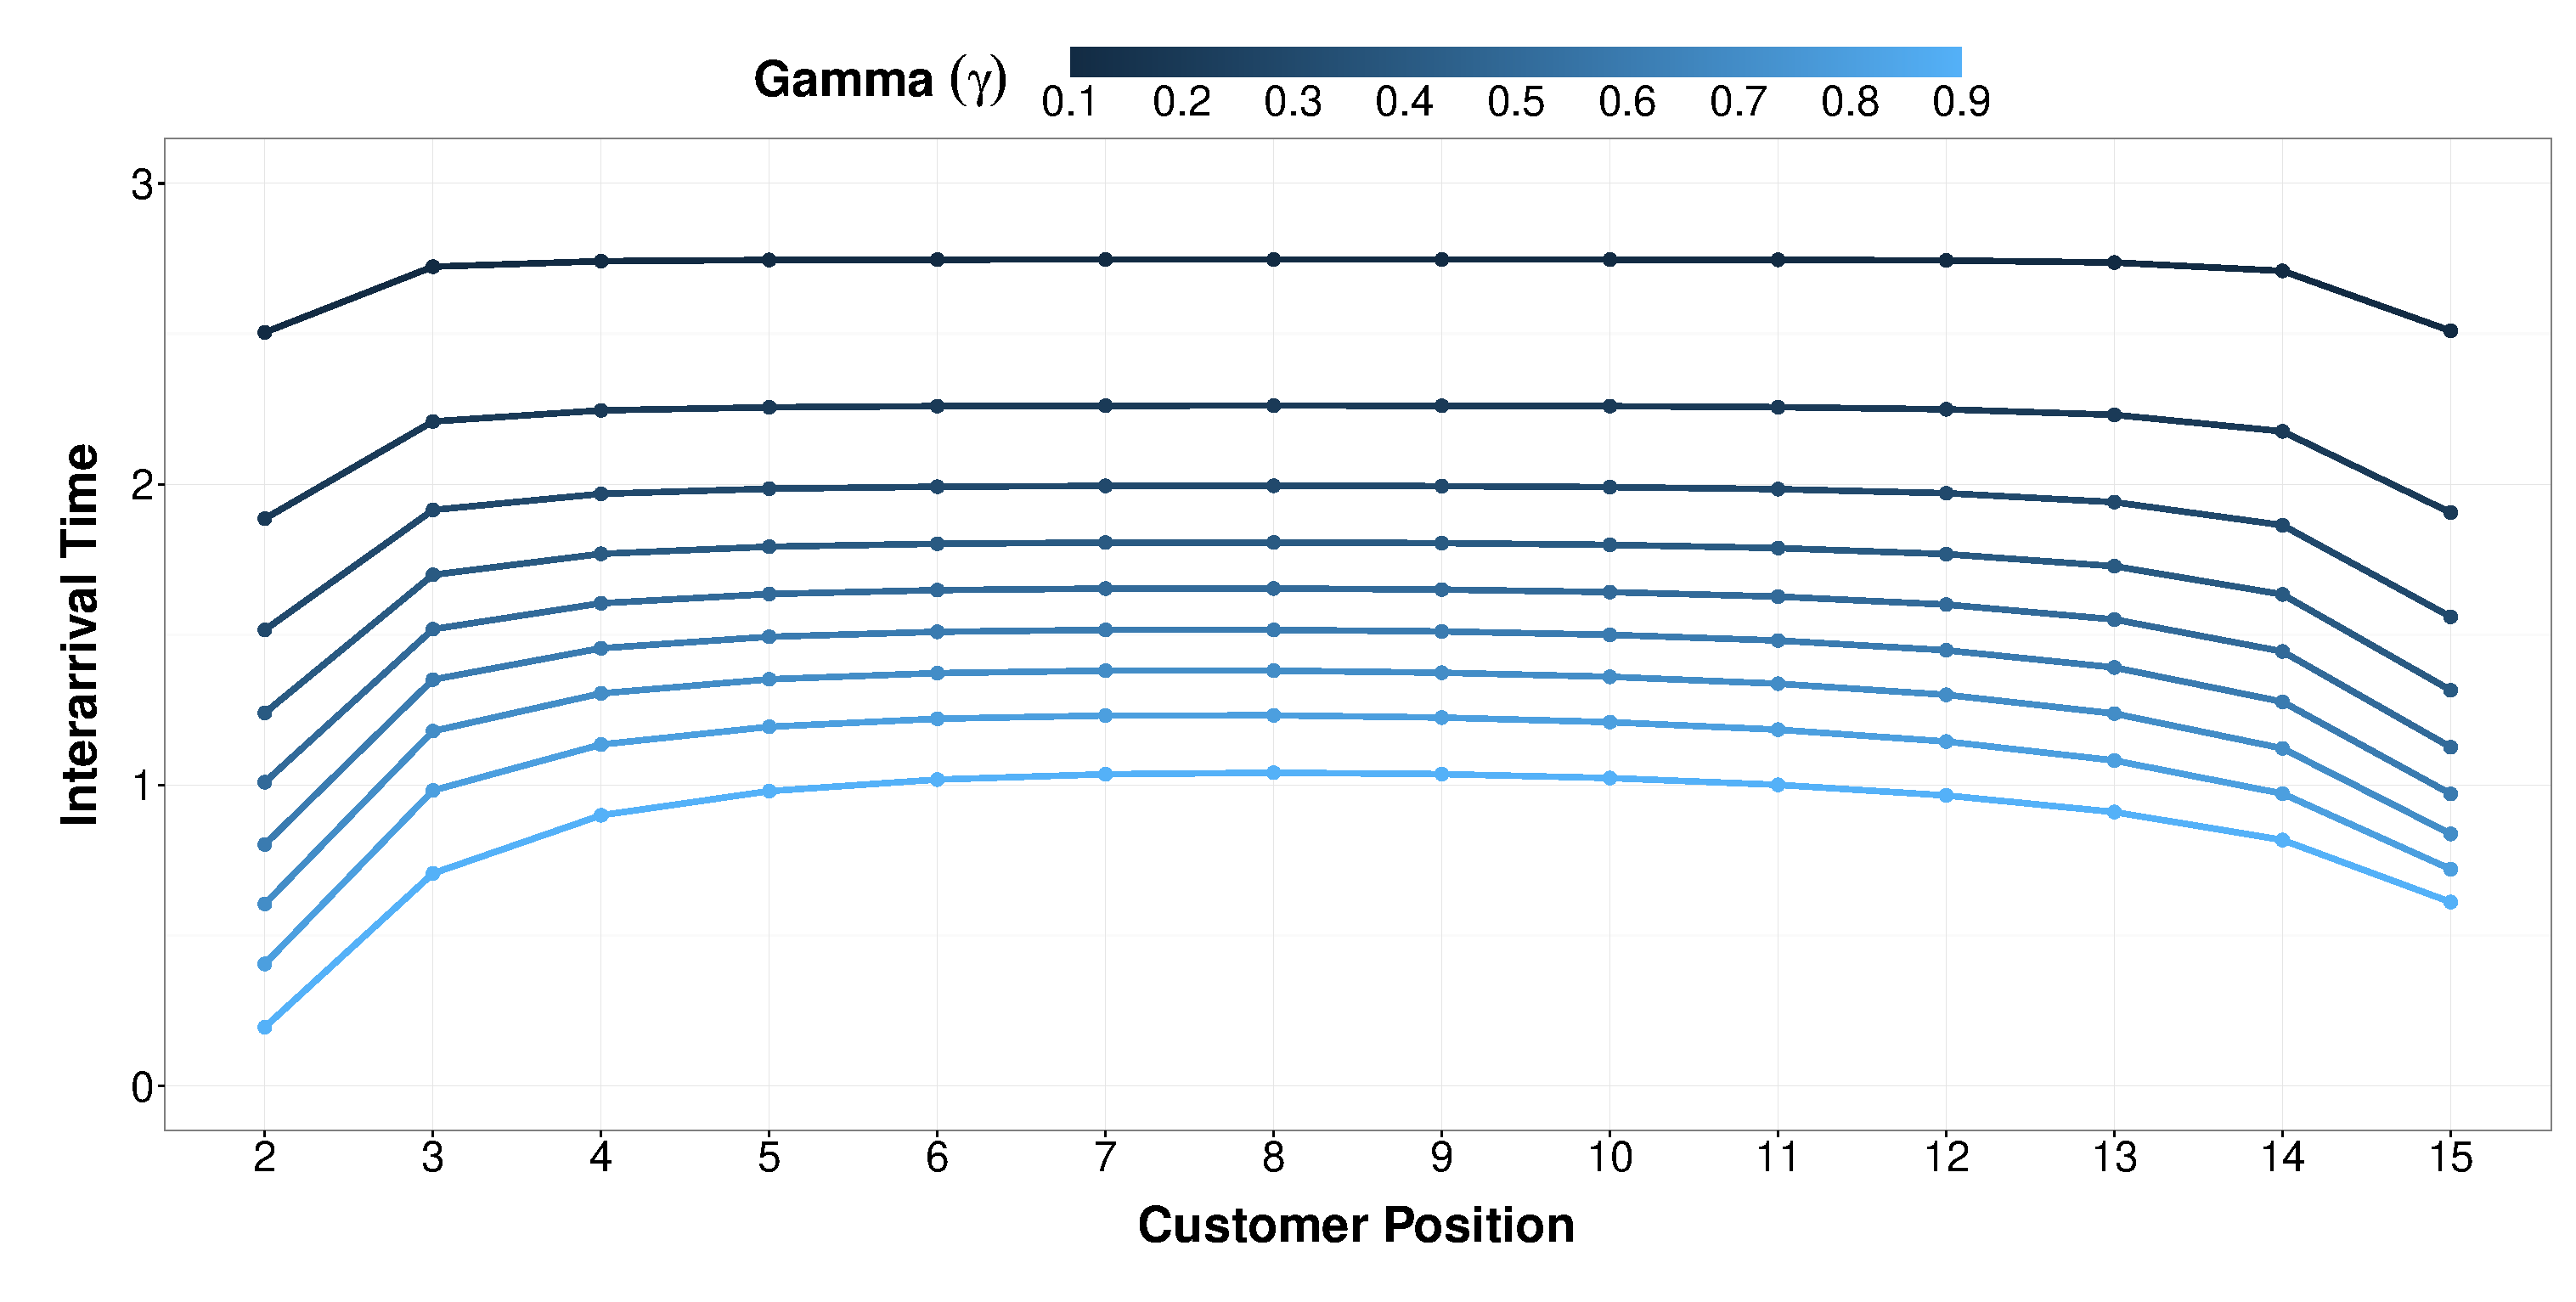
\includegraphics[width = 0.85\textwidth]{Static_Line_Interarrival_Gamma.eps}
	\caption{Optimal interarrival time for each of the $14$ customers after the first customer. Figure generated assuming $\mu = 1$. Each line is plotted for a fixed value of $\gamma = \frac{c_{S}}{c_{S} + c_{W}}$. The darkest line is for $\gamma = 0.1$. As $\gamma$ increases, the lines become lighter.}
	\label{fig:Static_Time_Gamma}
\end{figure}

The optimal interarrival times increase for the initial few customers, remain constant for the majority of customers, and then decrease for the last few customers. This is the dome-shape that was observed by \citet{Stein} and \citet{Mendel}. The observation that the first customers arrive close together obeys Bailey's Low that was first recommended by \citet{Bailey}. As $\gamma$ increases (i.e., the relative cost of server availability), the optimal interarrival times decrease while obeying the same general shape.

The common approach to efficiently finding the optimal static schedule involves simplifying the model by assuming a constant interarrival time (i.e., $x_{1} = \ldots = x_{n - 1}$). \citet{Stein} justify this simplification by claiming that for any single server queue with exponential service times, the average waiting time of a customer will be at a minimum for constant interarrival times. If this justification holds true, then this guarantees that constant interarrival times is optimal for $\gamma = 0$ (i.e., $c_{S} = 0$). However, it does not imply that it's optimal for $\gamma > 0$.

The constant interarrival simplification significantly reduces computation cost, but Figure~\ref{fig:Static_Time_Gamma} suggests that it is clearly not optimal for the first few and last few customers. In addition, it is not possible to include this simplification in the dynamic schedule model presented in the following chapter. Thus, this simplification is not pursued here.










































